%----------------------------------------------------------------
%
%  File    :  survey-basics.tex
%
%  Author  :  Julian Philipp Wolf, TU Graz, Austria
% 
%  Created :  14 May 2017
% 
%  Changed :  16 May 2017
% 
%----------------------------------------------------------------


\chapter{Basics}\label{chap:Basics}


This chapter explains the different types of graphs and their corresponding matrices, which techniques are used on matrices and how to interpret the resulting patterns.

\section{Definitions}
In mathematics a graph is an ordered pair $G = (V, E)$ containing a set of nodes $V$ and a set of edges $E$. However, some literature refers to nodes as ``vertices" (thus the $V$) or ``points".
Edges may be called ``arc" or lines. 
On the other hand, in the case of a directed graph, edges may also be called arrows. Moreover: \begin{itemize}
	\item $V$ is not allowed to be empty
	\item $E$ is allowed to be empty
	\item The \textbf{order} of a graph is the number of vertices $|V|$
	\item The \textbf{size} of a graph is the number of edges $|E|$
\end{itemize}

In this paper, every node in the graph has its distinctive unique id, which never changes. This holds for the reordering of the matrices too - when reordering rows and columns, the corresponding index stays with the column, otherwise the graph would be changed with this operation.


\section{Types of Graphs}

Basically, there are two types of edges (directed and undirected) and two types of cost calculations (weighted and unweighted), which leads to 4 different graphs. Figure~\ref{fig:graph_types} shows these 4 different types of graphs. 


\begin{table}[H]
  \centering
\begin{tabu}{cc}
	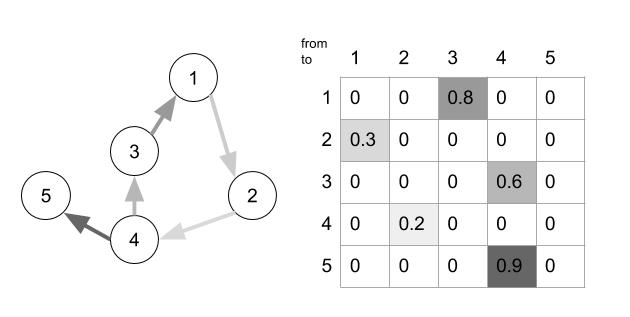
\includegraphics[width=0.49\textwidth]{images/directed_weighted_graph}
	 &
	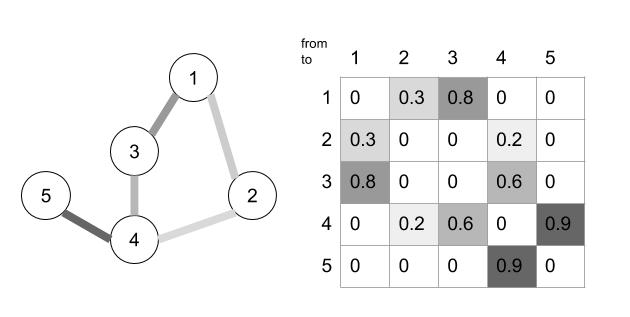
\includegraphics[width=0.49\textwidth]{images/undirected_weighted_graph} \\
	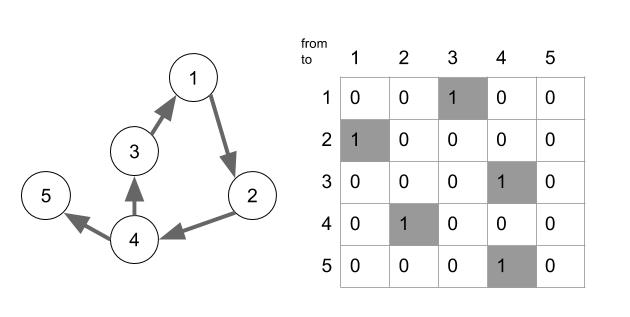
\includegraphics[width=0.49\textwidth]{images/directed_graph}  &
	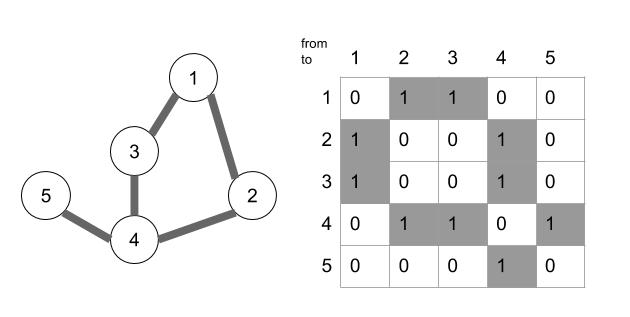
\includegraphics[width=0.49\textwidth]{images/undirected_graph} 
\end{tabu}
\captionof{figure}{4 different types of graphs (top: weighted directed and undirected, bottom: unweighted directed and undirected)\label{fig:graph_types}}
\end{table}


\subsection{Directed/Undirected}

Undirected edges may be traversed in any direction, whereas directed edges may just be traversed in one direction. For matrix representation of graphs, neither the mathematical \textbf{quiver}, a directed graph which has multiple arrows pointing from node $x$ to $y$, nor the \textbf{multigraph}, a graph which contains multiple undirected edges connecting just two nodes, is used.


\subsection{Weighted/Unweighted}

Graphs without costs defined for their edges, so called \textbf{unweighted graphs}, may be processed differently: 
\begin{itemize}
\item Either the algorithm searches for the shortest path, thus defining a uniform cost on all edges
\item Or there is no cost calculation at all, even the amount of edges is ignored
\end{itemize}

When adding weights to the edges, the graph is called a \textbf{weighted graph}. These weights typically represent different things, for example:
\begin{itemize}
\item time
\item length
\item energy consumption
\item elevations
\end{itemize}
to name just a few.

With weights defined on the edges, the approaches of algorithms are different, as the shortest path, in despite of number of traversed edges, is not necessarily the cheapest one. 



\section{Use cases}
Some use cases of the different graph types are (to name just a few examples):
\begin{itemize}
\item Navigation system (weighted directed)
	\begin{itemize}
		\item Nodes: cities/POIs
		\item Edges: routes directed (one way streets)
		\begin{itemize}
			\item weights
			\begin{itemize}
				\item length of street (find shortest way)
				\item time to traverse the street (find fastest way)
			\end{itemize}		
		\end{itemize}
	\end{itemize}		
\item Subway map (undirected unweighted)
\begin{itemize}
	\item Nodes: stations
	\item Edges: connections between stations
\end{itemize}
\item Relations of tweets (directed unweighted)
\begin{itemize}
	\item Nodes: single tweet entry
	\item Edges: references to other tweets
\end{itemize}
\end{itemize}


\section{Matrix Representation of Graphs}

When representing graphs in a matrix, an adjacency matrix is used. Adjacency matrices are structured with every row and every column representing one node. This leads to an N x N square matrix, where N is the number of nodes. 

These matrices show some patterns according to their corresponding graph but most times these patterns are not immediately visible. There are some techniques to reveal these patterns, all of them involving the reordering of the matrix.


\subsection{Reordering}

The main goal of reordering the matrix is to cluster the edges and thus reveal certain patterns. An example of this behavior can be seen in figure~\ref{fig:reorder}. 

\begin{figure}[h]
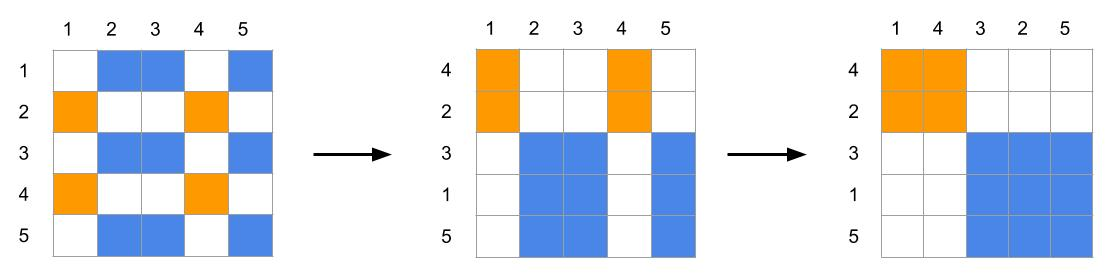
\includegraphics[width=\textwidth]{images/reorder}
\caption{Reordering a matrix\label{fig:reorder}}
\end{figure}


When reordering the matrix, the indices of the single rows and columns stay with the rows, otherwise the graph would change by this work step. In this example, at first the rows 1 and 4 get swapped and as a second step columns 2 and 4. In this way the full connection pattern of the two subgraphs may be observed. 

\subsection{Patterns}
There are 4 main patterns which may be revealed by reordering the matrix. These patterns can be combined in such a way, that for example a sub graph creates a circle, but one node if it is connected to every other node. This results in a combination of the star and the circle pattern. 
The four different patterns can be seen in the corresponding figures~\ref{fig:patterns}.

\begin{table}[H]
  \centering
\begin{tabu}{cc}
	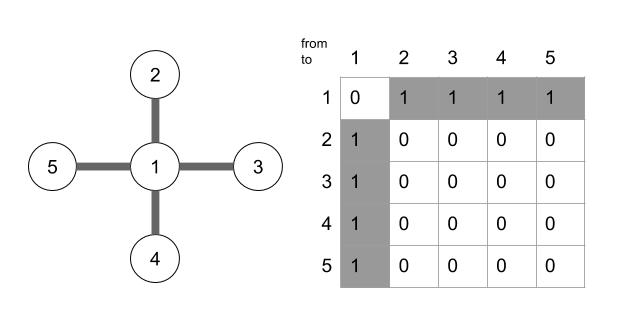
\includegraphics[width=0.49\textwidth]{images/pattern_star}  &
	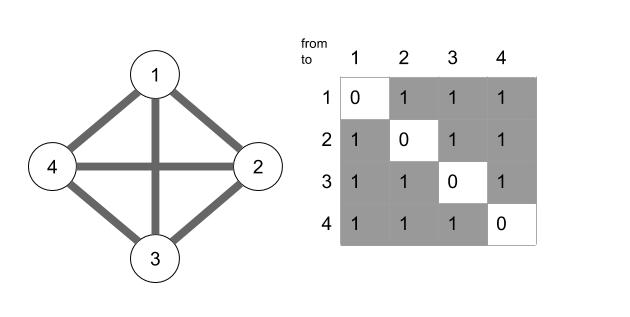
\includegraphics[width=0.49\textwidth]{images/pattern_full} \\
	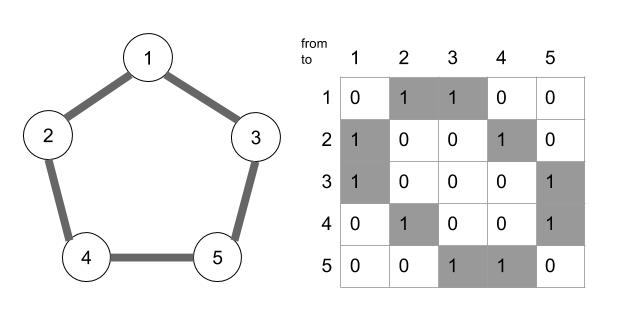
\includegraphics[width=0.49\textwidth]{images/pattern_circle} &
	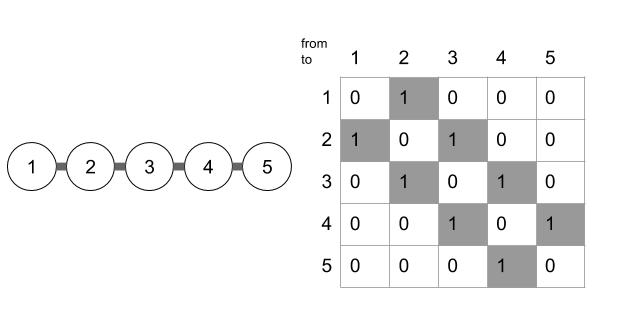
\includegraphics[width=0.49\textwidth]{images/pattern_line} 
\end{tabu}
\captionof{figure}{4 differnet patterns: star, full, circle and line\label{fig:patterns}}
\end{table}
